\section{Conceptos Preliminares}
\subsection{Acervo Genético, y Poblaciones Monomórficas y Dimórficas.}

El \textit{chemostat} o \textit{quimistato} es un dispositivo de laboratorio que está diseñado para el estudio del crecimiento de microorganismos en un ambiente controlado, en un medio líquido. Este dispositivo funciona de la siguiente forma: a un recipiente de vidrio cerrado, de entre 1 mL y unos pocos litros, se le suministra un medio fresco a través de una bomba de afluente. Para mantener un volumen constante, una segunda bomba extrae el líquido a la misma velocidad. Los microorganismos que han sido añadidos al recipiente únicamente pueden alimentarse del la bomba de afluente, y la tasa de crecimiento de esta está definida como la relación entre la tasa de afluente y el volumen del recipiente. Entre los sustratos y factores de crecimiento añadidos al medio, uno es el llamado sustrato de control, que limita el crecimiento \citep{chemostat}.

\begin{center}
	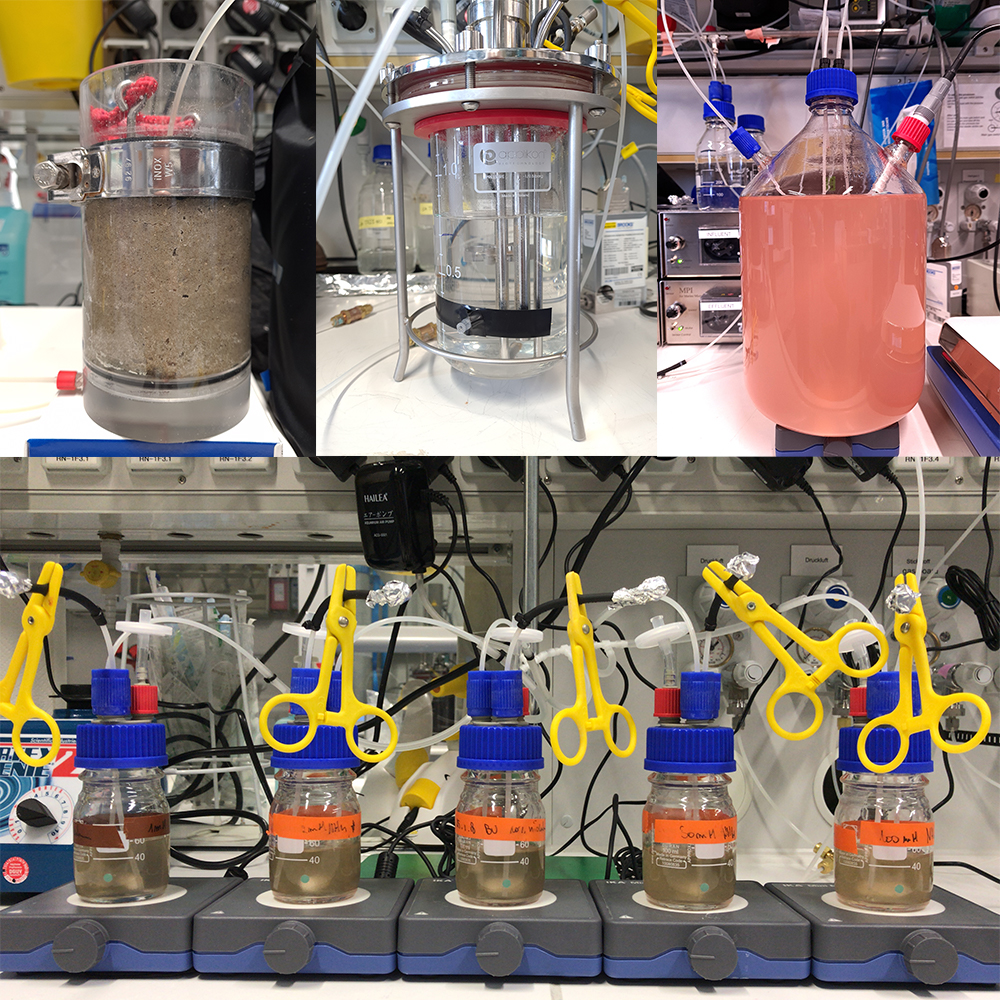
\includegraphics[scale=0.2]{Chemostat.jpg}
\end{center}

Algunas de las utilidades del quimiostato son que puede ser utilizado en cultivos puros para el estudio de la cinética del crecimiento microbiano, o para enfoques ómicos más detallados. También se puede utilizar para experimentos de competición \citep{chemostat}.

En estos experimentos se liberan en el recipiente dos o tres microorganismos diferentes, con nichos comparables en condiciones variables; con tasas de crecimiento altas o bajas; con concentraciones de oxígeno altas o bajas; distintos valores de pH o temperatura; con o sin factores de crecimiento, etc \citep{chemostat}.

\subsection{Ecuación de Hamilton-Jacobi.}

Desarrollamos la idea principal detrás de la ecuación con al que trabajaremos:

Sea una ecuación parcial diferencial no lineal \citep{evans} de la forma:
\begin{equation}\label{og}
	F(x;u,\nabla u)=0
\end{equation}

con $x\in\Omega\subseteq\Reals^n$, si renombramos $p\doteq\nabla u$ notación vectorial, asumimos que $F=F(x,u,p)$ es una función continua $F:\Reals^n$x$\Reals$x$\Reals^n \to \Reals$.

Dado $u(x)=\overline{u}(x)$ con $x\in\partial\Omega$ se construye una solución (al menos localmente, en la vecindad de la frontera) por el método de características.

Fijando un punto $x\in\partial\Omega$ considérese una curva parametrizada por $t:x(t)$ con $x(0)=y$, y con:
\begin{equation*}
	\begin{split}
		u(t) & \doteq=u(x(t))                \\
		p(t) & \doteq p(x(s))=\nabla u(x(t))
	\end{split}
\end{equation*}
Denotando por un punto la derivada con respecto a $t$ tenemos:
\begin{equation}\label{casi}
	\begin{split}
		\dot{u}  & =\sum_i \frac{\partial u}{\partial x_i}\dot x_i=\sum_i p_i \dot x_i \\
		\dot p_j & =\sum_i \frac{\partial^2 u}{\partial x_i\partial x_j} \dot x_i
	\end{split}
\end{equation}

Diferenciando \eqref{og} con respecto a $x_j$:

\begin{equation*}
	\begin{split}
		\frac{\partial F}{\partial x_j}+\frac{\partial F}{\partial u}\frac{\partial u}{\partial x_j}+\sum_i \frac{\partial F}{\partial p_i}\frac{\partial^2 u}{\partial x_i\partial x_j} & =0                                                                                   \\
		-\frac{\partial F}{\partial x_j}-\frac{\partial F}{\partial u}p_j                                                                                                                & =\sum_i \frac{\partial F}{\partial p_i}\frac{\partial^2 u}{\partial x_j\partial x_i}
	\end{split}
\end{equation*}

Al usar \eqref{casi} renombramos $\dot x_i=\frac{\partial F}{\partial p_i}$ obtenemos entonces:

\begin{equation*}
	\begin{split}
		\dot x_i & =\frac{\partial F}{\partial p_i}                                   \\
		\dot{u}  & =\sum_i p_i\frac{\partial F}{\partial p_i}                         \\
		\dot p_j & =-\frac{\partial F}{\partial x_j}-\frac{\partial F}{\partial u}p_j
	\end{split}
\end{equation*}

Que ahora, para un tipo específico de problema supongamos que $F$ no depende explícitamente de $u$, entonces recuperamos las ecuaciones canónicas de Hamilton y podemos escribir $F\to\Ham$, y en notación vectorial.
\begin{equation*}
	\begin{split}
		\dot x  & =\frac{\partial \Ham}{\partial p}        \\
		\dot{u} & =p\cdot \frac{\partial \Ham}{\partial p} \\
		\dot p  & =-\frac{\partial \Ham}{\partial x}
	\end{split}
\end{equation*}
con $x(0)=y$, $u(0)=u(y)$ y $p(0)=\nabla u(y)$.

De esta forma, podemos aplicar el formalismo de Hamilton-Jacobi a una variedad de problemas no necesariamente mecánicos, solamente pidiendo que la ecuación original cumpla $F=F(t;x,\nabla u)$.
